%----------------------------------------------------------------------------------------

% Define some commands to keep the formatting separated from the content 
\newcommand{\keyword}[1]{\textbf{#1}}
\newcommand{\tabhead}[1]{\textbf{#1}}
\newcommand{\code}[1]{\texttt{#1}}
\newcommand{\file}[1]{\texttt{\bfseries#1}}
\newcommand{\option}[1]{\texttt{\itshape#1}}
\newcommand{\grados}{$^{\circ}$}

%----------------------------------------------------------------------------------------
%\section{Introducción}
%----------------------------------------------------------------------------------------

% Chapter 1

\chapter{Introducción general} % Main chapter title
\label{Chapter1} % For referencing the chapter elsewhere, use \ref{Chapter1} 
\label{Intro}

Este capítulo introduce al lector a la motivación original del trabajo realizado. Se explica el marco de investigación del que forma parte este proyecto, se presentan los sistemas de información visual y también el estado del arte en controladores de carteles led para estos sistemas.\\

  


%En el capítulo 2 se introduce vocabulario técnico específico. Se presenta una descripción del sistema con el foco en la red de comunicaciones TCN, el sistema PIDS, sus interacciones y componentes.\\
%
%En el capítulo 3 se abordan cuestiones de diseño de sistema. Se especifican los requerimientos y casos de uso que se plantean en el espacio problema y también las consideraciones del espacio solución. Se detalla la solución en términos de arquitectura, patrones de software, descripción de componentes e implementación. Se incluye también los planos de los circuitos eléctricos del hardware existente que fueron relevados al realizar este trabajo.\\
%
%En el capítulo 4 se abordan cuestiones relacionadas al entorno real del sistema: visitas técnicas, mediciones realizadas, hardware ad-hoc realizado para las mediciones y un breve análisis de las tramas de datos de la red PIDS existente.\\
%
%En el capítulo 5 se tratan las conclusiones principales del desarrollo, su potencial fabricación en serie y los pasos a seguir para integrar al resto de ramales ferroviarios. En el apéndice de bibliografía se encontrarán las principales referencias técnicas, científicas e institucionales relevantes para este trabajo.\\


\section{Descripción del trabajo}

En este trabajo se desarrolla el sistema de control para carteles de matriz led del sistema de información visual para pasajeros (PIDS) de Trenes Argentinos. Las formaciones de Trenes Argentinos cuentan con carteles de matriz led en sus coches, en el frente y en el contrafrente del tren. Todos estos carteles se interconectan a través de una red de comunicaciones propia del PIDS, por la que también se transmiten distintos tipos de datos, como datos de mapas led, mensajes de audio, información para los carteles led e incluso videos de cámaras de seguridad. La red PIDS convive y se interconecta con la red de comunicaciones del tren (TCN), que es una red estándar. Además, en los buses de datos de la red TCN, se transmiten datos de sensores de velocidad, de frenado y eventos que indican apertura o cierre de puertas, entre otros. \\

Los carteles led del sistema PIDS suelen presentar fallas a lo largo de su ciclo de vida, lo que implica tareas de mantenimiento, reparación o reposición. Si bien existen muchos tipos de carteles led disponibles comercialmente, la integración al sistema de comunicaciones del tren es propietaria del fabricante de trenes. Para el caso de Trenes Argentinos, el proveedor está radicado en China, lo que hace muy costoso y lento el proceso de reposición o mantenimiento de equipamiento. Por esta razón, el desarrollo local de tecnología para sistemas PIDS es estratégico, ya que no solo fomenta la industria local, sino que también extiende la vida útil de los trenes.\\

%Esta necesidad motiva el desarrollo como búsqueda de autonomía tecnológica en áreas de vacancia que pueden ser cubiertas por el sistema científico-tecnológico nacional.

El eje de este trabajo es el desarrollo de un sistema a medida para Trenes Argentinos. La necesidad que prima es generar y brindar al personal de operaciones la información necesaria para construir y mantener los sistemas PIDS. Como resultado, este trabajo también tiene impacto directo en el pasajero, ya que contribuye a mejorar la calidad del servicio.\\


%\pagebreak
\section{Objetivos y alcance}

El  contexto de este trabajo se encuentra enmarcado en un Proyecto de Desarrollo Estratégico (PDE) de la Secretaría de Ciencia y Técnica de la Universidad de Buenos Aires (UBACyT). El PDE se titula PDE\_15\_2020 - "Sistema de monitoreo y gestión de la red TCN en formaciones ferroviarias" \citep{PDE-TCN}. Las partes que se involucran y forman parte del equipo de trabajo en este proyecto son el Grupo de Investigación en Calidad y Seguridad de las Aplicaciones Ferroviarias (GICSAFE), creado en 2017 en el marco del Consejo Nacional de Investigaciones Científicas y Técnicas (CONICET) de la República Argentina, y la  Operadora Ferroviaria Sociedad del Estado (SOFSE), también conocida como Trenes Argentinos Operaciones. El proyecto está orientado a cubrir necesidades tecnológicas concretas del sistema ferroviario argentino. Este tipo de proyectos son instrumentos de promoción científico-tecnológica que revalorizan e incrementan el aporte de la Universidad al desarrollo socioproductivo.\\

El objetivo principal de este trabajo es diseñar e implementar un sistema de información visual para pasajeros a bordo del tren. El sistema de información visual para pasajeros existente consta de una parte manual y una automática. Cuando el conductor del tren asume su puesto para prestar servicio (o toma cabina), programa en una pantalla cuáles van a ser las estaciones cabecera. Los nombres de estas estaciones cabecera se visualizan en las marquesinas del frente y contrafrente del tren, como puede verse en la figura \ref{fig:tren}.

\begin{figure}[ht]
	\centering
	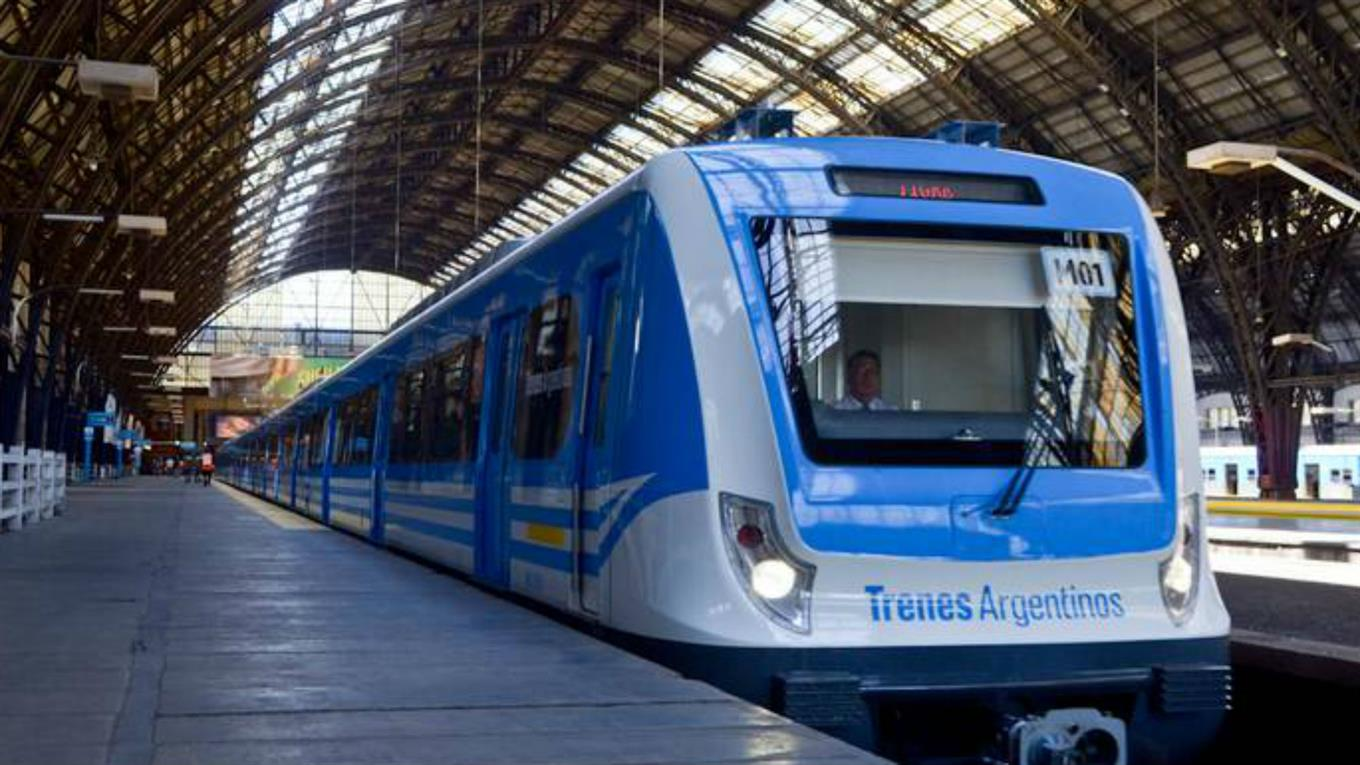
\includegraphics[width=1\textwidth]{./Figures/tren.jpg}
	\caption{Foto de una formación operativa de Trenes Argentinos. Se observa el cartel de matriz led frontal que indica el destino Tigre.}
	\label{fig:tren}
\end{figure}


En el interior de los coches, también hay carteles led. Estas marquesinas muestran mensajes a los pasajeros, como el nombre de la próxima estación o la estación arribada (por ejemplo, “Próxima estación Belgrano” o “Estás en estación Belgrano”). Ésta información se
presenta de manera automática basándose en variables de sistema que monitorean el detenimiento del tren, su velocidad y la apertura o cierre de puertas. Toda esta información, junto con otros datos de supervisición y control, se transmite a través de una red de comunicación interna del tren que se denomina TCN (\textit{Train Communication Network}) de acuerdo a las especificaciones definidas en el estándar\citep{IEC-61375-1999}. Este estándar define para la red TCN dos buses jerárquicos donde se conectan los subsistemas electrónicos: el WTB (\textit{Wire Train Bus}), que se utiliza para supervisar cambios topográficos en el tren y se conecta entre los vagones, y el MVB (\textit{Multi-Vehicle Bus}) \citep{CSN-EN-61375-2-1}\citep{IEC-61375-3-1:2012}, donde se conectan los sensores y actuadores de cada coche, como los sistemas de frenos, los controles de las puertas, los medidores de velocidad, el sistema de información, entre otros. Ambos buses utilizan interfaces eléctricas que se basan en redes RS485.\\


 El sistema propuesto en este trabajo tiene como objetivo captar los mensajes de información al pasajero que viajan por la red existente y presentarlos en un display led. El sistema se compone principalmente de cuatro partes:
 \begin{itemize}
\item Display led.
\item Placa de control.
\item Cableado de interconexión.
\item Firmware del sistema embebido
 \end{itemize}

El diagrama del prototipo se presenta en la figura \ref{fig:diagramaPIDSCIAA}. El display led matricial representa los carteles de los coches del tren. La placa de control se debe poder conectar a la entrada con al bus de la red RS485 que corresponda y a la salida con un display led matricial.

\begin{figure}[ht]
	\centering
	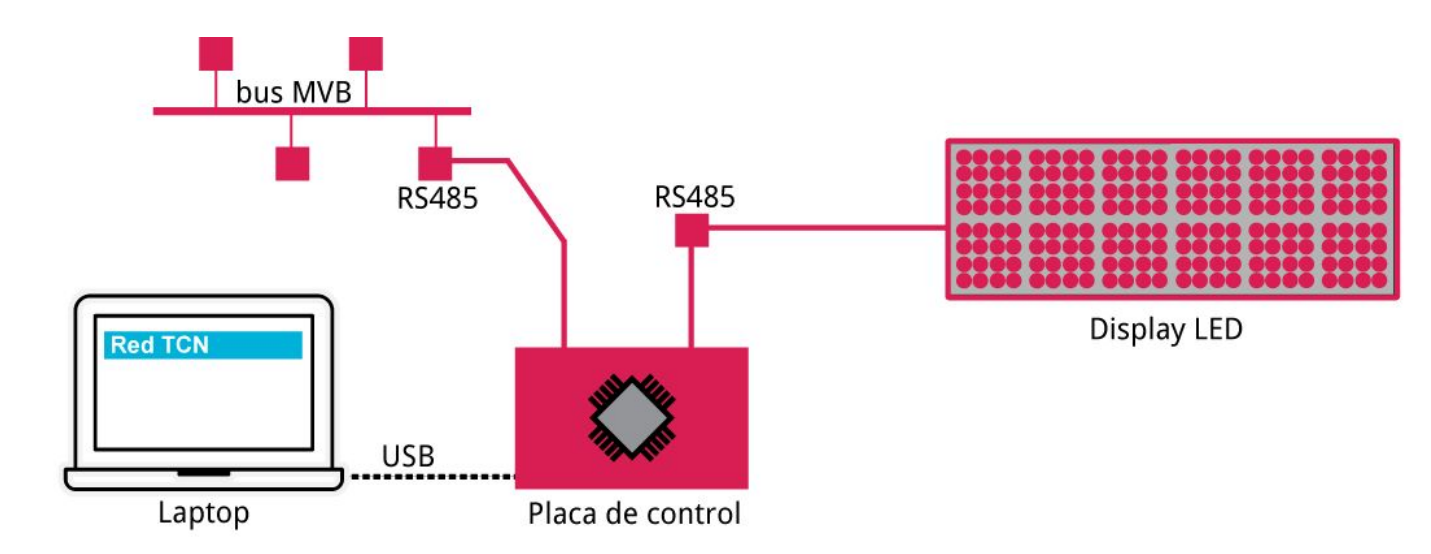
\includegraphics[width=1\textwidth]{./Figures/diagramaPIDSCIAA.png}
	\caption{Diagrama de bloques del sistema embebido propuesto basado en la plataforma EDU-CIAA.}
	\label{fig:diagramaPIDSCIAA}
\end{figure}


La placa de control está basada en la plataforma EDU-CIAA \citep{proyecto-ciaa} o en alguna de las plataformas desarrolladas por el CONICET-GICSAFe. La conexión entre el display y la placa así como de la placa con la red TCN deberá ser compatible con el estándar RS-485, definido como capa física de la red TCN. El
firmware a desarrollar se carga a la placa de control utilizando el puerto USB de una laptop. Este firmware es el responsable de leer los mensajes del sistema de información al pasajero y presentarlos en el display.\\

Las cualidades que debe satisfacer este proyecto son:
\begin{itemize}
\item Compatibilidad: debe ser compatible con el sistema PIDS existente.
\item Practicidad: debe ser de fácil uso para el personal de Trenes Argentinos Operaciones.
\end{itemize}

Este proyecto permitirá implementar las funciones de visualización del sistema de información al pasajero sin depender del equipamiento existente. El sistema actual es un equipamiento integrado y propietario, y este proyecto busca separar algunas de sus funciones, específicamente las relacionadas con la visualización de información para pasajeros, y presentarlas en un display led genérico. Por otro lado, permitirá reponer los carteles que en la actualidad quedan fuera de servicio por fallas o pérdida del material original y no pueden ser reparados. De esta manera, el valor principal que aporta este proyecto es contribuir con la sustitución de repuestos faltantes por medio de desarrollo y reducir la dependencia tecnológica de la empresa con los fabricantes. Este proyecto tiene impacto directo en las formaciones ferroviarias existentes, que brindan servicio a los pasajeros todos los días.\\

\section{Introducción a los sistemas de información visual}

Los sistemas de información visual para pasajeros están presentes en diversas industrias y aplicaciones. Se encargan de proveer información a pasajeros en  movimiento y tienen un rol fundamental en la industria del transporte.\\

 Las personas se trasladan por tierra o aire usando automóviles, ómnibus, subtes, trenes o aviones, entre otros. Los sistemas de información visual presentan necesidades y soluciones distintas en cada caso. Por ejemplo, en autopistas, se comunican accidentes u obras viales en ejecución usando carteles gigantes con información en tiempo real. En aeropuertos, los pasajeros aéreos acceden a información sobre llegada, el estado o la salida de vuelos. A los pasajeros de ómnibus, les interesa conocer los tiempos de espera y las líneas en operación al llegar a una estación. Los pasajeros de trenes utilizan estos sistemas para conocer el destino o la próxima estación cuando están viajando. Estos carteles pueden estar ubicados al aire libre o dentro de un recinto, pero en general,  requieren estar sincronizados con los vehículos en movimiento. \\

Los sistemas de información visual para pasajeros, constan principalmente de tres componentes: un sistema que genera datos, una red de transmisión y un sistema de pantallas. Las especificaciones de cada sistema varían según el ámbito de aplicación. Típicamente, en los trenes se requiere comunicación en tiempo real, lo que conlleva la adopción de protocolos de datos de tiempo real (RTP). En aplicaciones ferroviarias, también es fundamental garantizar la integridad, disponibilidad y confiabilidad de los datos. Además, existen otros requerimientos de carácter operativo, como el mantenimiento y la facilidad de instalación. Estos últimos aspectos son esenciales en la operación de una formación ferroviaria y tienen impacto directo en el ciclo de vida de un tren.\\

 Los sistemas PIDS instalados en los trenes se interconectan con una red TCN. Ésta última, sigue un estándar que define tanto las interfaces eléctricas como los protocolos de comunicación. En la red TCN, se conectan dispositivos para el sensado y control de frenos, de puertas, de monitoreo, entre otros, usando una arquitectura jerárquica de buses de datos. La red TCN representa un estándar robusto, maduro, probado y con gran adopción internacional. Sin embargo, los sistemas PIDS se presentan sin la necesidad de ser compatibles con los estándares de TCN, al menos hasta la revisión del año 2005. Existen diversas soluciones comerciales de sistemas PIDS, para aplicaciones de entretenimiento por ejemplo, pero se requiere de un trabajo de integración adicional para que funcionen en un tren.\\
 
 En este trabajo se introduce una breve descripción de las redes TCN y su evolución en el tiempo. Para el caso de las formaciones de Trenes Argentinos, que forman el marco de este trabajo, se presenta también el detalle de interconexión TCN-PIDS, el desarrollo de un sistema de control para los carteles led del sistema PIDS y los resultados de las pruebas de campo realizadas en conjunto con la empresa Trenes Argentinos Operaciones (SOFSE). Se ha organizado esta memoria buscando acercar al lector primero los conceptos principales de la aplicación y luego el detalle técnico del diseño del sistema embebido propuesto. \\

\section{Estado del arte}

En esta breve sección, se resumen algunas características y aspectos comunes de los sistemas PIDS, tanto para sistemas ferroviarios como para sistemas de transporte integrados. En lugar de ser un estudio sistemático, la intención es guiar al lector en las consideraciones que fueron tenidas en cuenta en este trabajo. En primer lugar, se describe el rol que juegan estos sistemas y una noción de su mercado, mencionando aquellos proveedores que se consideraron relevantes por claridad en la información, marca global y diseño conceptual de la solución. Luego, se describen algunas soluciones comerciales innovadoras, y finalmente se presenta en tablas algunos aspectos técnicos comunes en distintas soluciones. Adicionalmente, se mencionan algunos trabajos académicos relevados. Se han elegido como dimensiones de análisis las funcionalidades y servicios que debe ofrecer un sistema PIDS, las características principales de la oferta de carteles electrónicos, y por último las características técnicas de las unidades de control. \\


El cliente de mayor impacto de los servicios que provee un sistema PIDS es la red de transporte (trenes, subtes, metros, ómnibus) de una gran ciudad, debido a su masividad. En términos generales, se observa que las empresas que proveen sistemas PIDS a las redes metropolitanas de transporte de las grandes ciudades lo hacen bajo formatos distintos. Algunas empresas instalan televisores o pantallas de video, otras carteles led, otras incluyen carteles impresos con algún elemento indicador tipo led, o bien leds en forma de flecha mezclándose con la señalización para indicar nombres de estaciones, pantallas led para desplegar publicidad entre mensajes, etcétera. En algunos países, se han realizado esfuerzos durante la última década para que los sistemas PIDS faciliten el acceso a la información del transporte para personas con discapacidades, movilidad reducida y de edad avanzada. Actualmente, los sistemas PIDS se diseñan teniendo en cuenta al pasajero en el centro de todo, buscando ofrecer servicios de información que mejoren la experiencia de viaje.\\

\begin{figure}[h!]
	\centering
	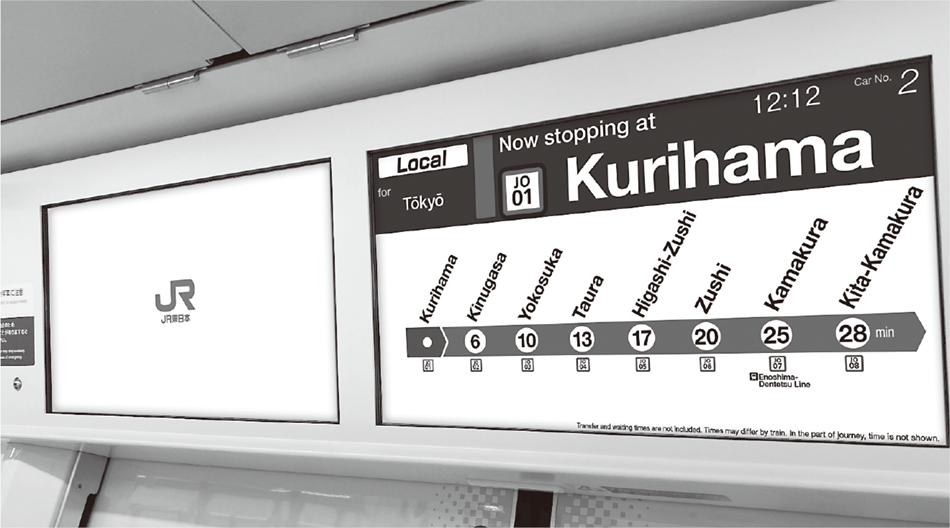
\includegraphics[width=0.49\textwidth]{./Figures/HitachiCartelPIDS.png}
	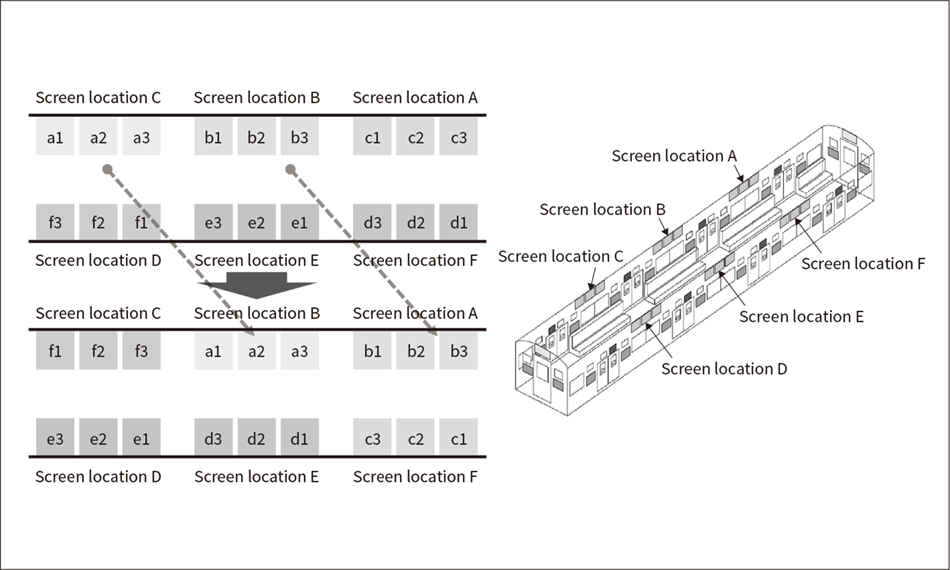
\includegraphics[width=0.49\textwidth]{./Figures/HitachiDisplayArray.png}
	\caption{Solución de carteles para sistemas PIDS de Hitachi. Consultado en \citep{Hitachi}}
	\label{fig:Hitachi}
\end{figure}

Hitachi ofrece una solución para publicidad que consiste en tres pantallas en array, que se sincronizan para formar una sola y transmitir video con conectividad WiMAX. Cada uno de estos arreglos se posicionan arriba de las ventanas en ambos lados de los coches, alcanzando el despliegue de hasta dieciocho pantallas sincronizadas por coche, como se puede ver en la figura \ref{fig:Hitachi}. De esta manera, logran transmitir varios mensajes distintos en simultáneo a los pasajeros sin que tengan que moverse de su asiento.\\


Por otro lado, Toshiba ofrece una solución que permite transmitir publicidad e información al pasajero en una misma pantalla LCD en simultáneo. La solución está centrada en la pantalla como dispositivo central, ofreciendo pantallas de 32\" y 42\", de 1920 x 540 píxeles, full color de hasta 16,7 millones de colores, com amplio ángulo de visión y de gran luminancia\citep{Toshiba}. En la mayoría de los casos, las soluciones ofrecidas buscan cubrir tanto la demanda de un sistema PIDS como la oferta de publicidad de cara al pasajero, como es habitual en las estaciones y formaciones ferroviarias.\\



\begin{figure}[h]
	\centering
	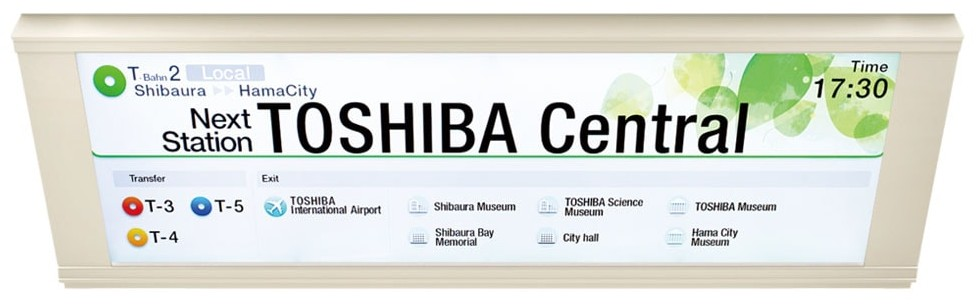
\includegraphics[width=0.49\textwidth]{./Figures/ToshibaPIDS.jpg}
	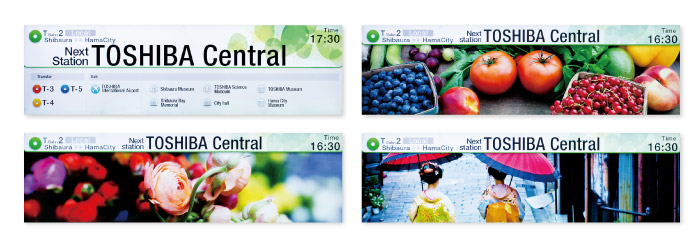
\includegraphics[width=0.49\textwidth]{./Figures/ToshibaDisplayColorOpciones.jpg}
	\caption{Solución de displays LCD para sistemas PIDS de Toshiba.Consultado en \citep{Toshiba}}
	\label{fig:Toshiba}
\end{figure}


El grupo austríaco Trapeze \citep{Trapeze} distingue cuatro tecnologías principales en sistemas PIDS: Led, LCD, canales móviles o apps, y e-ink que es una tecnología de LCD monocromo relativamente nueva. Al seleccionar carteles, es importante considerar varios factores, como los ángulos de visión, las condiciones del ambiente donde van instalados (por ejemplo, si estarán a la intemperie o requerirán visibilidad con la luz del sol), el tamaño o resolución de los caracteres en pantalla, la selección de colores y su relación con la capacidad estadística de visión de los pasajeros, el diseño mecánico, el acceso a controles para personas con movilidad reducida, la fuente de alimentación eléctrica y la capacidad de realizar actualizaciones de sistema de forma remota. \\ 


\begin{figure}[h]
	\centering
	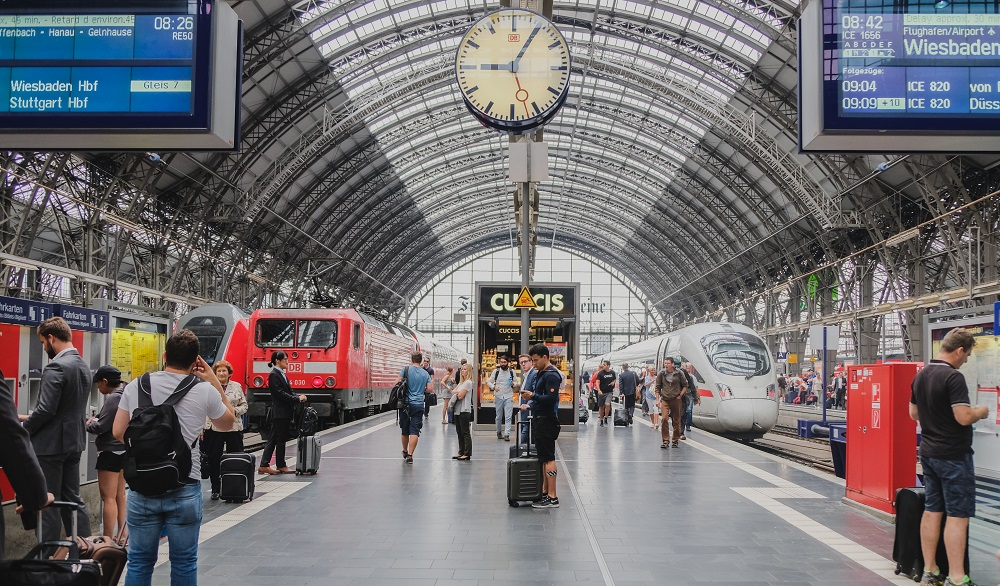
\includegraphics[width=0.32\textwidth]{./Figures/TrapezeStation.jpg}
	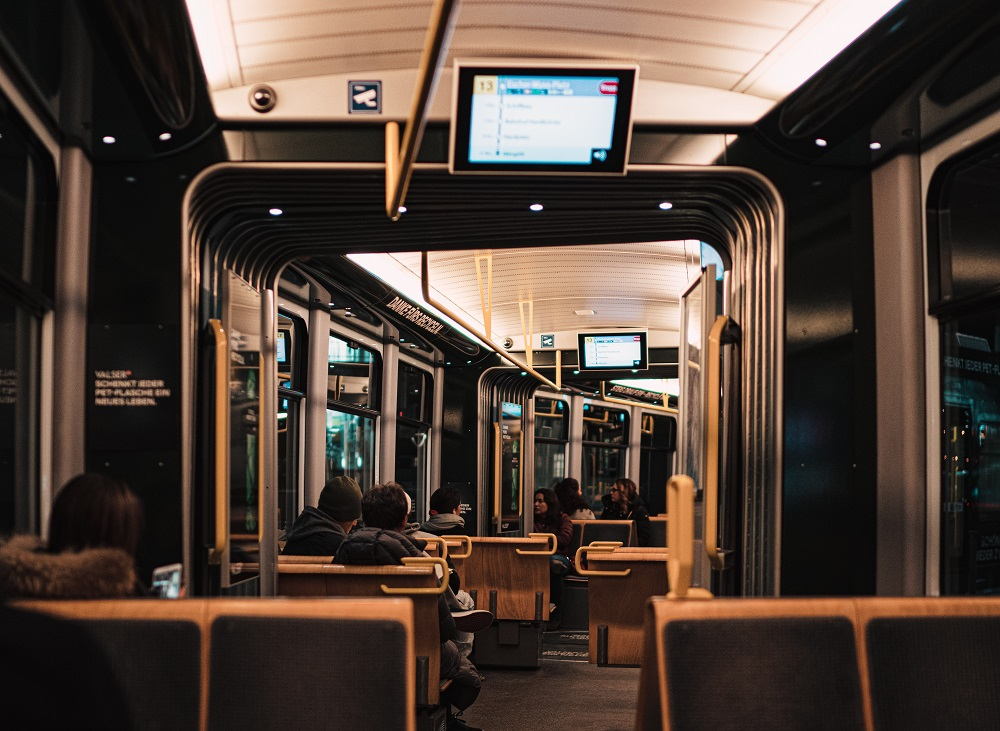
\includegraphics[width=0.32\textwidth]{./Figures/TrapezeOnboard.jpg}
	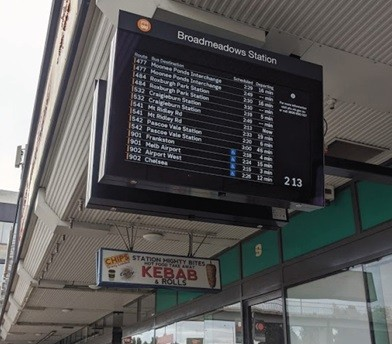
\includegraphics[width=0.32\textwidth]{./Figures/TrapezeTimetable.jpg}
	\caption{Sistema PIDS del proveedor austríaco Trapeze. Consultado en \citep{Trapeze}}
	\label{fig:Trapeze}
\end{figure}

Además, se sugiere la importancia de la precisión en la información que ofrece como servicio el sistema PIDS. Si un pasajero recibe el número de andén incorrecto al llegar a la estación muy probablemente perderá el tren, resultando en una mala experiencia de viaje. La capacidad de interconectar el sistema PIDS con otros canales de información, especialmente en puntos nodales de transporte, también ofrece mayores beneficios al usuario final. Si un pasajero puede anticiparse y ver el tiempo estimado entre una línea de omnibus o de tren antes de llegar a la estación donde hace combinación, entonces puede tomar una mejor elección basada en datos ofrecidos por el sistema PIDS. Estos y otros aspectos de sistema centrados en el usuario se resumen en la tabla \ref{tab:tablaSistemasPIDS}.\\


\begin{table}[ht]
\caption[Caption for LOF]{Principales aspectos y servicios asociados a sistemas PIDS\protect\footnotemark}
%\caption{Principales aspectos y servicios asociados a sistemas PIDS\footnote{Elaboración del autor.}.}
\begin{tabular}{ll}
\hline
\textbf{Conectividad} &\begin{tabular}[c]{@{}l@{}}
    RS-485, serial, USB.                    \\
    Ethernet, fibra óptica, coaxil.         \\
    Wi-Fi, WiMax, GPS.                      \\
    2G / 3G / 4G / 5G.                      \\
\end{tabular}\\ \hline
\textbf{Interconexión} &\begin{tabular}[c]{@{}l@{}}
    App del tren, horarios programados.     \\
    Ómnibus, información multinodal.        \\
    Portales de noticias, publicidad.       \\
    Canal de información estatal.           \\
\end{tabular}\\ \hline
\textbf{Accesibilidad} &\begin{tabular}[c]{@{}l@{}}
    Información por audio, ángulos de visión de los carteles. \\
    Facilidades para personas en sillas de ruedas. \\
    Facilidades para personas de edad avanzada. \\
    Correcto y cuidado sistema de señalización. \\
\end{tabular}\\ \hline
\textbf{Información} &\begin{tabular}[c]{@{}l@{}}
   Estimación de tiempos y aviso de cortes en tiempo real.\\
   Correcto trackeo de vehículos y conexiones.            \\
   Mensajes de alerta o precauciones, números de emergencia.\\
\end{tabular}\\ \hline
\textbf{Mantenibilidad} &\begin{tabular}[c]{@{}l@{}}
   Fácil instalación, bajo costo de reposición.\\
   Consumo eléctrico.                          \\
   Actualizaciones de software.                \\
\end{tabular}\\ \hline
\end{tabular}
\label{tab:tablaSistemasPIDS}
\end{table}

\footnotetext{Fuente: elaboración propia del autor.}

Desde el punto de vista centrado en los carteles, se consideran varias especificaciones importantes de los sistemas PIDS, como las dimensiones del cartel, la densidad de píxeles por unidad de área, la cantidad de colores o leds por píxel, los niveles de intensidad lumínica, el brillo y contraste, la potencia eléctrica. Entre estas especificaciones típicas de los carteles de los sistemas PIDS, el ángulo de visión es una de las variables más consideradas ya que en sistemas PIDS implican el alcance a mayor cantidad de pasajeros de la información en pantalla. En la tabla \ref{tab:tablaDisplays} se presenta un resumen de estas características. Las fuentes consultadas para la elaboración de esta tabla son diversos portales internacionales de distribución de componentes electrónicos.\\



\begin{table}[h!]
\caption[Caption for LOF]{Principales características de displays para sistemas PIDS\protect\footnotemark}
\label{tab:tablaDisplays}
\begin{tabular}{|l|l|l|l|l|}
\hline
\textbf{Display}
    & \textbf{led matricial}      
    & \textbf{led RGB}      
    & \textbf{TFT LCD}   
    & \textbf{LCD RGB}  \\ 
\hline
\textbf{Colores}  
    & \begin{tabular}[c]{@{}l@{}}
        monocromo \\ 
        bicolor   \\ 
        tricolor  \\ 
        multicolor \\ 
        (<10 colores)
    \end{tabular} 
    & \begin{tabular}[c]{@{}l@{}}
        desde 256 \\ 
        hasta 16,7 M\\ 
        (típicamente)\end{tabular}   
    & hasta 16,7 M    
    & \begin{tabular}[c]{@{}l@{}}
        16.7M \\ 
        (típicamente)\\ 
        1,000 M\end{tabular}\\ 
\hline
\textbf{\begin{tabular}[c]{@{}l@{}}
Ángulo \\ de visión\end{tabular}}       
    & 110º     
    & 160º   
    & 120º-140º      
    & 178º      \\ 
\hline
\textbf{\begin{tabular}[c]{@{}l@{}}
Intensidad \\ cd/m$^2$\end{tabular}}   
    & 450 
    & 1500-2000       
    & 350 
    & 900 \\ 
\hline
\textbf{\begin{tabular}[c]{@{}l@{}}
Densidad \\ de píxeles\end{tabular}}    
    & \begin{tabular}[c]{@{}l@{}}
        3,9 k\\ 
        27,7 k\\ 
        110 k\\ 
        *\end{tabular}    
    & \begin{tabular}[c]{@{}l@{}}
        P16: 3,9 k\\ 
        P12: 6,9 k\\ 
        P10: 10 k\\ 
        P8: 15,6 k\\ 
        P6: 27,7 k\\ 
        P5: 40 k\\ 
        P4: 62,5 k\\ 
        P3: 111 k\\ 
        P2.5: 160 k\\ 
        P2: 250 k\\ 
        *\end{tabular} 
    & \begin{tabular}[c]{@{}l@{}}
        29 M/m$^2$ \\ 
        Pixel size\\ 
        179 x 192 um\end{tabular} 
    & \begin{tabular}[c]{@{}l@{}}
        4,26 M/m$^2$\\ 
        Pixel size \\ 
        484 x 484 um\\
        \\ 
        29 M/m$^2$ \\ 
        Pixel size \\ 
        179 x 192 um\end{tabular} \\ 
\hline
\textbf{Potencia} 
    & 10 W          
    & 15-316 W   
    & 20 W    
    & 25 W \\ 
\hline
\end{tabular}
\end{table}


\footnotetext{Fuente: elaboración propia del autor.}

Cada cartel requiere de un controlador como interfaz para procesar información y la codifica según la lógica que requiera el tipo de cartel. Los controladores de los carteles de matriz led suelen basarse en circuitos digitales, en microcontroladores de 8, 16 o 32 bits o en FPGA. Las tasas de transmisión de datos requieren señales de clock que pueden variar desde algunos kHz hasta cientos de MHz. Los tamaños del buffer de memoria depende de la cantidad de píxeles que tenga la pantalla. Las interfaces físicas pueden ser periféricos de un microcontrolador, un pin de propósito general o bien puertos USB o HDMI. Los carteles LCD en muchos casos requieren de la transmisión de señales de video. Esto implica mayores costos de implementación que la alternativa led, pero también mayor versatilidad en la programación de contenidos. En la tabla \ref{tab:tablaControladores} se resumen algunas características principales de los requerimientos de los controladores.\\

\begin{table}[h!]
\caption[Caption for LOF]{Principales características de controladores de uso general para aplicaciones PIDS\protect\footnotemark}
\label{tab:tablaControladores}
\centering
\begin{tabular}{|l|l|l|l|}
\hline
\textbf{\begin{tabular}[c]{@{}l@{}}Unidad de \\ procesamiento\end{tabular}} & \textbf{MCU 8/16/32 bits}                                                                       & \textbf{FPGA / ASIC / DSP}                                                        & \textbf{CPU / DSP}                                                                                      \\ \hline
\textbf{Clock}                                                              & 1-200 MHz                                                                                       & 10-250 MHz                                                                        & 1-3 GHz                                                                                                 \\ \hline
\textbf{Memory buffer}                                                      & 1 kB                                                                                            & 1-512 MB                                                                          & 1-10 GB                                                                                                 \\ \hline
\textbf{Conectividad}                                                       & \begin{tabular}[c]{@{}l@{}}UART (1-4)\\ USB (1-2)\\ RS485\\ GPIO (1-20)\\ Ethernet\end{tabular} & \begin{tabular}[c]{@{}l@{}}Pmod\\ I/O pins (20-800)\\ Ethernet\\ USB\end{tabular} & \begin{tabular}[c]{@{}l@{}}USB \\ VGA\\ HDMI\\ DVI\\ display Port\\ PCI / PCI-E\\ Ethernet\end{tabular} \\ \hline
\textbf{Programación}                                                       & C / C++/ Assembly                                                                               & VHDL, Verilog, XML                                                                & \begin{tabular}[c]{@{}l@{}}C, C++, Java, \\ Python, XML\end{tabular}                                    \\ \hline
\end{tabular}
\end{table}

\footnotetext{Fuente: elaboración propia del autor.}

Una vez instalados, los sistemas PIDS suelen requerir mantenimiento. Muchas veces hay fallas de hardware, como por ejemplo leds que dejan de funcionar, una fuente de alimentación o una memoria que se debe reemplazar. Otras veces se requieren cambios en el software, por ejemplo actualizar el contenido de un mensaje o bien cambiarlo. Los atributos de mantenibilidad, versatilidad, modularidad y confiabilidad en la implementación pueden tener un impacto económico relevante en la operación de un servicio de transporte. Para líneas de trenes que cuentan con muchas formaciones ferroviarias operando en simultáneo, las tareas de actualización pueden ser muy intensivas en términos de horas de trabajo y requerir también capacitaciones técnicas periódicas al personal de mantenimiento. Incluso no todos los dispositivos pueden recibir actualizaciones en producción, esto es, en la locación física donde funcionan. En muchos casos es necesario desinstalarlos, llevarlos a un centro técnico y actualizarlos fuera de operación, lo que requiere de ventanas de mantenimiento y de tiempos reducidos para realizar tareas que pueden ser susceptibles a errores. Otra forma es enviar un técnico al sitio que pueda conectar algún periférico y actualizar manualmente cada dispositivo.\\

De los trabajos académicos relevados se mencionan aquellos con propuestas del sistema de control que representan distintas tecnologías. En \citep{song2011design} se utiliza el chip AT89C52 para enviar caracteres chinos sobre matrices de 32 x 192 leds de un solo color; en \citep{liu2011design} se implementa una pantalla led RGB de 320 x 240 píxeles que rota 360º, permitiendo visualizar imágenes en color por persistencia de visión; en \citep{kurdthongmee2004design} se desarrollan algoritmos sobre FPGA usando búferes de datos para controlar una pantalla led de 160 x 32 píxeles alcanzando 32.768 colores; en \citep{lin2021active} se presenta el control de un micro display de transistores de película delgada (TFT) usando modulación por ancho de pulso (PWM) alcanzando 256 niveles de color a una frecuencia de refresco de 60 Hz, basado también en FPGA; en \citep{gago2009control} se presenta el control de píxeles virtuales para matrices led multicolor usando flip-flops tipo D. \\


En el diseño e implementación del presente trabajo, los carteles son de matriz led de un solo color y de distintas dimensiones (8 x 64, 32 x 64, 32 x 128). El control de los carteles tiene como factor común el uso del conjunto de chips digitales 74HC138, 74HC595 y 74HC245. La topología permite interconectar paneles en serie para construir carteles led de distinto tamaño usando la misma lógica de control. \\


